\chapter{Gramatici formale}
\label{ch:gramatici}

Pentru a vedea care este intuiţia din spatele conceptului de gramatici formale, vom porni de la exemplul următor. Să presupunem că se dă o mulţime de cuvinte:

\textit{ \{ casa, străluceşte, repede, copila, stă, frumos, câinele, aleargă, bine \} }

Şi trebuie să formăm propoziţii de câte trei cuvinte care să aibă înţeles în limba română. Dacă am alege la întâmplare cele trei cuvinte, atunci avem toate şansele de a forma propoziţii care nu au niciun înţeles, cum ar fi, de exemplu:

\textit{ "repede casa bine" }

Pentru a elimina astfel de situaţii, am putea proceda în felul următor. Ştim că o propoziţie are sens dacă ea exprimă o acţiune, adică dacă are ceea ce gramatica limbii române numeşte \textit{predicat}. Această acţiune ar putea fi realizată de către cineva. Gramatica limbii române îl numeşte pe acest cineva \textit{subiect}. În plus, acţiunea ar putea să fie caracterizată într-un anume fel, gramatica limbii române numind această caracterizare \textit{complement circumstanţial de mod}. Printr-o astfel de judecată, am stabilit practic o structură a propoziţiilor cu sens, pe care le putem forma pornind de la o mulţime de cuvinte. Să notăm atunci această structură sub forma unei înlocuiri:

\textit{ Start $\rightarrow$ Subiect Predicat Complement }

Apoi, să grupăm cuvintele din mulţimea dată, în funcţie de partea propoziţiei care ar putea să fie. De exemplu, $casa, copila, câinele$ ar putea fi subiecte. Putem scrie aceasta tot sub forma unei înlocuiri:

\textit{ Subiect $\rightarrow$ casa | copila | câinele }

Analog putem proceda şi pentru predicat, şi pentru complement. În acest mod vom obţine patru înlocuiri cu ajutorul cărora, pornind de la Start, putem obţine o propoziţie cu sens folosind cuvintele din mulţimea dată.

\textit{ Start $\rightarrow$ Subiect Predicat Complement }

\textit{ Subiect $\rightarrow$ casa | copila | câinele }

\textit{ Predicat $\rightarrow$ străluceşte | stă | aleargă }

\textit{ Complement $\rightarrow$ repede | frumos | bine }

Mulţimea de cuvinte de la care am plecat, împreună cu mulţimea de elemente ajutătoare (\textit{\{ start, subiect, predicat, complement\}}) şi împreună cu cele patru înlocuiri de mai sus formează o gramatică formală. Observăm deci că o gramatică formală este un instrument care permite descrierea şi analiza unui limbaj, pe baza unei mulţimi de reguli, care prezintă modul în care se construiesc propoziţiile valide (şi numai acestea) din limbajul ţintă.

\section{Gramatici formale}

În continuare vom prezenta sintaxa gramaticilor formale. Pentru aceasta este nevoie să definim operatorii steluţa Kleene şi plusul Kleene.

Fie V o mulţime de simboluri (un alfabet). Definim, prin inducţie, următoarele mulţimi:
\begin{itemize}
\item
$V_{0} = \{ \epsilon \}$,
\item
$V_{1} = V$,
\item
$\dots$
\item
$V_{i+1} = \{ wv | w \in V_{i} \;, \; v \in V \}, \forall i > 0$.
\end{itemize}

\begin{definitie}
Operatorul \textbf{steluţa Kleene} asupra unei mulţimi V este definit astfel:

\[V^{*} = \mathop{ \cup }_{i \in \mathbb{N}} V_{i} = \{ \epsilon \} \cup V_{1} \cup V_{2} \cup V_{3} \cup \dots \]
\end{definitie}

\begin{definitie}
Definiţia operatorului \textbf{plusul Kleene} asupra unei mulţime V este:

\[V^{+} = \mathop{ \cup }_{i \in \mathbb{N} \setminus \{0\} } V_{i} = V_{1} \cup V_{2} \cup V_{3} \cup \dots \]
\end{definitie}

Altfel spus, $V^{*}$ este mulţimea tuturor şirurilor de simboluri peste $V$, iar $V^{+}$ este mulţimea tuturor şirurilor de simboluri peste $V$ cu excepţia şirului vid.

\begin{definitie}
O \textbf{gramatică} formală este un cvadruplu $G = (V_{N}, \Sigma, S, P)$, unde:
\begin{itemize}
\item
$V_{N}$ se numeşte mulţimea neterminalelor,
\item
$\Sigma$ se numeşte mulţimea terminalelor,
\item
S este simbolul iniţial (sau simbolul de start), $S \in V_{N}$,
\item
P este mulţimea regulilor de producţie, ale cărei elemente au forma:

$V^{*}V_{N}V^{*} \rightarrow V^{*}$, unde $V = V_{N} \cup \Sigma$ se numeşte alfabetul gramaticii.
\end{itemize}
\end{definitie}

Exemplu:

Fie gramatica $G = (V_{N}, \Sigma, S, P)$, astfel încât:

\begin{itemize}
\item
$V_{N}$ = \{Subiect, Predicat, Propoziţie\},
\item
$\Sigma$ = \{Ana, Ion, învaţă, doarme, ., ' '\},
\item
S este simbolul de start și anume Propoziţie,
\item
$P = \{$
\begin{itemize}
\item
Propoziţie $\rightarrow$ Subiect ' ' Predicat .,
\item
Subiect $\rightarrow$ Ana | Ion,
\item
Predicat $\rightarrow$ învaţă | doarme
\end{itemize}
\}
\end{itemize}

Iată convenţiile de notaţie care vor fi folosite de-a lungul lucrării:
\begin{itemize}
\item
literele mici de la începutul alfabetului latin (a, b, c, $\dots$) reprezintă elemente din mulţimea $\Sigma$ (simboluri terminale),
\item
literele mici de la sfârşitul alfabetului latin (u, v, x, $\dots$) reprezintă elemente din mulţimea $\Sigma^{*}$ (şiruri de simboluri terminale),
\item
literele mari de la începutul alfabetului latin (A, B, C, $\dots$) reprezintă elemente din $V_{N}$ (simboluri neterminale),
\item
literele mari de la sfârşitul alfabetului latin (U, V, X, $\dots$) reprezintă elemente din $V_{N} \cup \Sigma$ (simboluri terminale sau neterminale),
\item
literele alfabetului grecesc reprezintă şiruri din $(V_{N} \cup \Sigma)^{*}$ (şiruri de simboluri terminale şi neterminale).
\end{itemize}

Din exemplele de gramatici furnizate se poate observa că o gramatică formală definește numai lexicul (vocabularul) și sintaxa propozițiilor unui limbaj. Ea nu permite definirea semanticii propozițiilor unui limbaj. De asemenea, din definiția unei gramatici se poate observa că aceasta cuprinde lexicul (vocabularul) acestui meta-limbaj, precum și sintaxa regulilor de producție, însă nu cuprinde și semantica regulilor de producție. Aceasta va fi definită implicit prin definirea relației de derivare. În continuare vom prezenta semantica gramaticilor formale.

Fie $M$ o mulţime. Orice mulţime de perechi ordonate $R = \{ (a, b)| \; a,b \in M \}$, se numeşte relaţie binară peste $M$ ($R \subseteq A \times A$).

\begin{definitie}
Fie o gramatică $G = (V_{N}, \Sigma, S, P)$. \textbf{Derivarea într-un pas (derivarea directă)} este o relaţie binară între şiruri din $V^{*}$ notată cu $\Rightarrow$ ($\Rightarrow \subseteq V^{*} \times V^{*}$) şi definită astfel:

$\alpha \Rightarrow \beta$ dacă şi numai dacă $\alpha = xpy$ şi $\beta = rqt$, $x,p,y,r,q,t \in V^{*}$ şi $\exists \; p \rightarrow q \in P$.
\end{definitie}

Exemplu (pe baza gramaticii anterioare):

Subiect ' ' Predicat . $\Rightarrow$ Ana ' ' Predicat .

\begin{definitie}
Fie o gramatică $G = (V_{N}, \Sigma, S, P)$. \textbf{Derivarea în k paşi} este o relaţie binară între şiruri din $V^{*}$ notată cu $\Rightarrow^{k}$ şi definită astfel:

$\gamma \Rightarrow^{k} \delta$ dacă şi numai dacă $\exists \; \alpha_{1}, \alpha_{2}, \dots \alpha_{k+1}$ astfel încât $\alpha_{1} = \gamma, \alpha_{k+1} = \delta$ şi $\alpha_{i} \Rightarrow \alpha_{i+1}, \forall \; i \in [1,k]$.
\end{definitie}

Exemplu (pe baza gramaticii anterioare):

Subiect ' ' Predicat . $\Rightarrow$ Ana ' ' Predicat .

\begin{definitie}
\textbf{Închiderea tranzitivă a relaţiei de derivare} se notează $\Rightarrow^{+}$ şi se defineşte folosind relaţia de derivare în k paşi, astfel:

$\gamma \Rightarrow^{+} \delta$ dacă şi  numai dacă $\exists \; k \geq 1$ astfel încât $\gamma \Rightarrow^{k} \delta$.
\end{definitie}

\begin{definitie}
\textbf{Închiderea tranzitivă şi reflexivă a relaţiei de derivare} se notează $\Rightarrow^{*}$ şi se defineşte folosind închiderea trazitivă a relaţiei de derivare, astfel:

$\gamma \Rightarrow^{*} \delta$ dacă şi  numai dacă $\gamma = \delta$ sau $\gamma \Rightarrow^{+} \delta$.
\end{definitie}

\begin{definitie}
O \textbf{formă propoziţională} peste o gramatica $G = (V_{N}, \Sigma, S, P)$ se defineşte recursiv (inductiv) în modul următor:
\begin{enumerate}
\item
\textbf{S} este o formă propoziţională.
\item
Dacă $\textbf{aBt}$ este o formă propoziţională şi dacă există o regulă de producţie $B \rightarrow r \in P$, atunci $\textbf{art}$ este o formă propoziţională.
\end{enumerate}
\end{definitie}

Exemplu:

Propoziţie; Subiect Predicat.; Ana Predicat.; Subiect învaţă.; Ana învaţă.

\begin{definitie}
O forma propoziţională peste o gramatică G, care conţine numai simboluri terminale, se numeşte \textbf{propoziţie} generata de G.
\end{definitie}

Exemplu:

Ana învaţă.; Ion doarme.

Forma propoziţională şi propoziţia pot fi definite şi folosind relaţia de derivare. Dăm mai jos şi aceste două definiţii.

\begin{definitie}
O \textbf{formă propoziţională} peste o gramatica $G = (V_{N}, \Sigma, S, P)$ este orice şir $\alpha \in V^{*}$ cu proprietatea că $S \Rightarrow^{*} \alpha$.
\end{definitie}

Forma propoziţională este deci orice succesiune de simboluri terminale şi/sau neterminale care poate fi obţinută pornind de la simbolul de start prin 0 sau mai multe derivări.

\begin{definitie}
O \textbf{propoziţie} peste o gramatica $G = (V_{N}, \Sigma, S, P)$ este orice şir $x \in \Sigma^{*}$ cu proprietatea că $S \Rightarrow^{+} x$.
\end{definitie}

Propoziţia este deci orice succesiune de simboluri terminale care poate fi obţinută pornind de la simbolul de start prin cel puţin o derivare.

\begin{definitie}
Limbajul generat de o gramatica $G = (V_{N}, \Sigma, S, P)$ se notează cu L(G) şi reprezintă mulţimea tuturor propoziţiilor care pot fi generate de către această gramatică:

$L(G) = \{ x \in \Sigma^{*} | S \Rightarrow^{+} x \}$.
\end{definitie}

Exemplu:

$L(G) = \{$Ana învaţă., Ion învaţă., Ana doarme., Ion doarme.$\}$

O gramatica este o reprezentare finită (toate elementele sale sunt finite) a unui limbaj care poate să fie infinit. Nu orice limbaj are o reprezentare finită, cu alte cuvinte nu pentru orice limbaj există o gramatică care să îl reprezinte. Dacă este posibilă o astfel de construcţie, atunci pentru un acelaşi limbaj dat, se pot construi mai multe gramatici distincte care să îl genereze.

Singura modalitate prin care, pe baza unei gramatici, se pot genera propoziții cu un număr oarecare de simboluri este recursivitatea. Aceasta poate să apară la nivelul regulilor de producție și poate să fie recursivitate stanga ($A \Rightarrow^{*} A \alpha$) sau recursivitate dreapta ($A \Rightarrow^{*} \alpha A$), recursivitate directă ($A \rightarrow A \alpha$ și $A \rightarrow \alpha A$) sau recursivitate indirectă ($A \rightarrow \gamma B \beta, B \Rightarrow^{*} A \alpha$ și analog pentru recursivitatea dreapta).

De exemplu, fie gramatica $G = (V_{N}, \Sigma, S, P)$, astfel încât:

\begin{itemize}
\item
$V_{N}$ = \{Subiect, Predicat, Propoziţie, Frază\},
\item
$\Sigma$ = \{Ana, Ion, învaţă, doarme, ., ' '\},
\item
S este simbolul de start și anume Frază,
\item
$P = \{$
\begin{itemize}
\item
Frază $\rightarrow$ Propoziţie Frază | Propoziţie
\item
Propoziţie $\rightarrow$ Subiect ' ' Predicat .,
\item
Subiect $\rightarrow$ Ana | Ion,
\item
Predicat $\rightarrow$ învaţă | doarme
\end{itemize}
\}
\end{itemize}

Pe baza acestei gramatici se pot genera fraze care sunt formate din una, două sau un număr oarecare de propoziții.

Atunci când derivăm o formă propoziţională, putem ajunge în situaţia în care aceasta să conţină mai multe simboluri neterminale. Prin urmare va trebui să alegem pentru care dintre simbolurile neterminale vom aplica următoarea regulă de producţie pentru a face o derivare directă. Dacă într-o astfel de situaţie se alege întotdeauna neterminalul cel mai din stânga, atunci derivarea se va numi \textit{derivare stânga}. Dacă îl alegem întotdeauna pe neterminalul cel mai din dreapta, atunci derivarea se va numi \textit{derivare dreapta}.

Exemplu: 

Fie gramatica $G = (V_{N}, \Sigma, S, P)$, astfel încât:

\begin{itemize}
\item
$V_{N}$ = \{E\},
\item
$\Sigma$ = \{+, -, *, /, (, ), id\},
\item
S este neterminalul E,
\item
$P = \{$
\begin{itemize}
\item
E $\rightarrow$ E + E,
\item
E $\rightarrow$ E - E,
\item
E $\rightarrow$ E * E
\item
E $\rightarrow$ E / E
\item
E $\rightarrow$ (E)
\item
E $\rightarrow$ id
\end{itemize}
\}
\end{itemize}

Următorul şir de derivări, care reprezintă generarea propoziţiei \textit{id * (id + id)}, este format din derivări stânga.
\[ S \Rightarrow E * E \Rightarrow \textbf{id} * E \Rightarrow id * (E) \Rightarrow id * (E + E) \Rightarrow id * ( \textbf{id} + E) \Rightarrow id * ( id + id) \]

Pentru aceeaşi propoziţie, următorul şir de derivări este format din derivări dreapta.
\[\begin{multlined}[t]
S \Rightarrow E * E \Rightarrow E * \textbf{(E)} \Rightarrow E * (\textbf{E + E}) \Rightarrow E * (E + \textbf{id}) \\ \Rightarrow E * ( \textbf{id} + id) \Rightarrow \textbf{id} * ( id + id)
\end{multlined}\]

\section{Ierarhia Chomsky}

Ierarhia Chomsky este o ierarhie de clase de limbaje formale, care arată ce relaţie de incluziune există între acestea. Ierarhia a fost descrisă pentru prima dată de către lingvistul Naom Chomsky, într-un articol publicat în anul 1956. Apartenenţa unui limbaj la unul dintre tipurile ierarhiei se determină în funcţie de forma pe care o au regulile de producţie ale unei gramatici care generează limbajul respectiv. Din această cauză, ierarhia Chomsky poate fi văzută şi ca o ierarhie de clase de gramatici formale.

\begin{figure}[H]
\centering
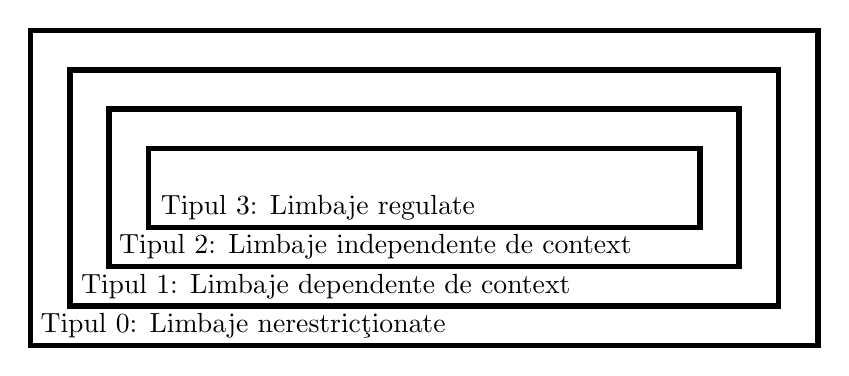
\begin{tikzpicture}
    \draw[line width=2] (0, 0) rectangle (10, 4) ;
    \draw (2.7, 0.25) node {Tipul 0: Limbaje nerestricţionate} ;
    
    \draw[line width=2] (0.5, 0.5) rectangle (9.5, 3.5);
    \draw (3.75, 0.75) node {Tipul 1: Limbaje dependente de context} ;
    
    \draw[line width=2] (1, 1) rectangle (9, 3);
    \draw (4.38, 1.25) node {Tipul 2: Limbaje independente de context} ;
    
    \draw[line width=2] (1.5, 1.5) rectangle (8.5, 2.5);
    \draw (3.65, 1.75) node {Tipul 3: Limbaje regulate} ;
\end{tikzpicture}
\label{FiguraIerarhiaChomsky}
\caption{Ierarhia Chomsky}
\end{figure}

Primul tip de gramatici din ierarhia Chomsky este tipul 0 şi este reprezentat de către \textbf{gramaticile nerestricţionate}. Nicio restricţie nu este impusă asupra regulilor de producţie ale unei astfel de gramatici.

Un limbaj este limbaj de tipul 0, dacă şi numai dacă el este generat de către o gramatică de tipul 0.

Gramaticile de tipul 1 sunt gramaticile dependente de context.

\begin{definitie}
O gramatică $G = (V_{N}, \Sigma, S, P )$ se numeşte \textbf{gramatică dependentă de context} dacă şi numai dacă \textbf{toate} regulile sale de producţie au forma $\alpha A \beta \rightarrow \alpha \gamma \beta$, unde $A \in V_{N}$, $\alpha, \beta \in V^{*}$ şi $\gamma \in V^{+}$.
\end{definitie}

Observaţie: Unii autori permit şi regulile de producție de forma $S \rightarrow \epsilon$ în cadrul mulţimii regulilor de producţie ale unei gramatici dependente de context, însă cu condiţia ca $S$ să nu apară în partea dreaptă a niciunei reguli de producţie.

Un limbaj este dependent de context, dacă şi numai dacă el este generat de către o gramatică dependentă de context.

Exemplu: 

Fie gramatica $G = (V_{N}, \Sigma, S, P )$, unde:

\begin{itemize}
\item
$V_{N} = \{$ Propoziţie, Subiect, Atribut, Predicat, Complement, Substantiv, Verb, Adjectiv, Adverb$\}$,
\item
$\Sigma = \{$ a merge, a cânta, este, face, copilul, câinele, frumos, rău, bine, mult, ., ' '$\}$,
\item
S este Propoziţie,
\item
$P = \{$
\begin{itemize}
\item
Propoziţie $\rightarrow$ Subiect [Atribut] Predicat [Complement].,
\item
Subiect $\rightarrow$ Substantiv | Verb,
\item
Atribut $\rightarrow$ Adjectiv,
\item
Predicat $\rightarrow$ Verb,
\item
Complement $\rightarrow$ Adverb,
\item
Verb Atribut $\rightarrow$ a merge Atribut | a cânta Atribut,
\item
Verb Complement $\rightarrow$ este Complement | face Complement,
\item
Substantiv $\rightarrow$ copilul | câinele,
\item
Adjectiv $\rightarrow$ frumos | rău,
\item
Adverb $\rightarrow$ bine | mult
\end{itemize}
$\}$
\end{itemize}

Gramaticile de tipul 2 sunt gramaticile independente de context.

\begin{definitie}
O gramatică $G = (V_{N}, \Sigma, S, P )$ se numeşte \textbf{gramatică independentă de context} dacă şi numai dacă \textbf{toate} regulile sale de producţie au forma $A \rightarrow u$, unde $A \in V_{N}$ şi $u \in V^{*}$.
\end{definitie}

Un limbaj este independent de context, dacă şi numai dacă el este generat de către o gramatică independentă de context.

Gramaticile regulate reprezintă gramaticile de tipul 3.

\begin{definitie}
O gramatică $G = (V_{N}, \Sigma, S, P )$ se numeşte \textbf{gramatică liniară dreapta} dacă este o gramatică independentă de context în care fiecare regulă de producţie este de forma $A \rightarrow a$ sau de forma $A \rightarrow aB$ sau de forma $A \rightarrow \epsilon$, unde $a \in \Sigma$, iar $A, B \in V_{N}$.
\end{definitie}

\begin{definitie}
O gramatică $G = (V_{N}, \Sigma, S, P )$ se numeşte \textbf{gramatică liniară stânga} dacă este o gramatică independentă de context în care fiecare regulă de producţie este de forma $A \rightarrow a$ sau de forma $A \rightarrow Ba$ sau de forma $A \rightarrow \epsilon$, unde $u \in \Sigma$, iar $A, B \in V_{N}$.
\end{definitie}

\begin{definitie}
O gramatică se numeşte \textbf{gramatică regulată} dacă este o gramatică liniară dreapta sau stânga.
\end{definitie}

Un limbaj este regulat dacă şi numai dacă el este generat de către o gramatică regulată.

Acum că am văzut definiţia pentru fiecare tip de limbaj/gramatică în parte, putem să explicăm semnificaţia ierarhiei Chomsky. După cum am precizat la începutul secţiunii, ierarhia Chomsky arată relaţia de incluziune dintre cele patru clase de limbaje definite. Prin urmare putem spune că: orice limbaj regulat este şi un limbaj independent de context; orice limbaj independent de context este şi un limbaj dependent de context; şi orice limbaj dependent de context este şi un limbaj nerestricţionat. Analog, putem spune că: nu orice limbaj nerestricţionat este şi un limbaj dependent de context; nu orice limbaj dependent de context este şi limbaj independent de context; şi nu orice limbaj independent de context este şi limbaj regulat.

Având în vedere restricţiile impuse asupra regulilor de producţie ale fiecărui tip de gramatici formale, se observă că limbajele regulate sunt cele mai simple, iar limbajele nerestricţionate sunt cele mai complexe. Cu alte cuvinte, complexitatea limbajelor scade de la tipul 0 către tipul 3. Iată câte un exemplu de limbaj pentru fiecare clasă în parte. Limbajele naturale sunt limbaje de tipul 0. Limbajele de programare sunt limbaje de tipul 2. (De fapt, unele aspecte ale limbajelor de programare le-ar clasifica ca şi limbaje de tipul 1, însă în practică se preferă definirea lor prin gramatici independente de context, adăugându-se câteva restricţii suplimentare.) Limbajul atomilor lexicali ai unui limbaj de programare (cuvintele cheie, numele de funcţii, variabile, structuri, clase, ş.a., constantele numerice, constantele literale, constantele de tip şir de caractere, operatorii, semnele de punctuaţie) este un limbaj de tipul 3.

Am văzut că gramaticile formale permit definirea limbajelor prin generare. Adică, pornind de la simbolul de start, prin derivări succesive, putem genera orice propoziţie a limbajului definit de gramatica respectivă. Cum se poate rezolva problema inversă? Fiind dată o propoziţie oarecare, cum se poate stabili dacă ea aparţine unui anumit limbaj (definit de o gramatică dată)? Pentru aceasta se foloseşte un "dispozitiv" capabil sa recunoască dacă o propoziţie dată aparţine sau nu limbajului pe care el îl defineşte. În capitolul introductiv am arătat că astfel de dispozitive sunt automatele finite. 

Pentru fiecare clasă de limbaje în parte, s-a propus câte un model matematic al unui dispozitiv capabil să facă acest lucru, astfel: pentru limbajele regulate, acest lucru se poate face cu ajutorul unui automat finit, pentru limbajele independente de context este nevoie de un automat finit cu stivă, pentru limbajele dependente de context este nevoie de o maşină Turing cu bandă limitată, iar pentru limbajele nerestricţionate este nevoie de o maşină Turing.

Scopul acestui curs este prezentarea teoriei traducerii/compilării pentru limbajele de programare. Limbajele de programare pot fi definite prin gramatici independente de context, iar vocabularul unui limbaj de programare este un limbaj regulat. De aceea ne vom opri numai asupra analizei pentru limbajele regulate şi pentru cele independente de context.

\section{Arbori sintactici}

Fie $M$ o mulţime de noduri şi $R$ o relaţie binară peste M. Atunci $G=(M, R)$ se numeşte \textbf{graf orientat}. Dacă $(a, b) \in R$, atunci definim următoarele mulţimi:
\begin{itemize}
\item
$input(a) = \{ b | (b, a) \in R \}$,
\item
$output(a) = \{ b | (a, b) \in R \}$.
\end{itemize}

\textbf{Un arbore} este un graf orientat $(M, R)$ cu următoarele restricţii:
\begin{itemize}
\item
$\exists \; r \in M$ unic, astfel încât $input(r) = \emptyset$,
\item
$\forall \; a \in M, \; a \neq r, \; card(input(a)) = 1$,
\item
$\forall \; a \in M, \; (r, a) \in R^{*}$.
\end{itemize}

\begin{definitie}
Fie o gramatică formală $G = (V_{N}, \Sigma, S, P )$. Un \textbf{arbore de derivare} (arbore sintactic) $A=(M, R)$ este un arbore etichetat ordonat de la stânga la dreapta cu proprietăţile:
\begin{enumerate}
\item
rădăcina arborelui este etichetată cu $S$,
\item
pentru orice nod $a \in M$ cu descendenţi, astfel încât A este eticheta nodului $a$, iar $X_{1}, X_{2}, \dots, X_{i}$ sunt etichetele descendenţilor lui a, $\exists \; A \rightarrow X_{1} X_{2} \dots X_{i} \in P$.
\end{enumerate}
\end{definitie}

Exemplu:

Arborele sintactic corespunzător propoziţiei \textit{Ana învaţă.} este următorul:

\begin{figure}[H]
\centering
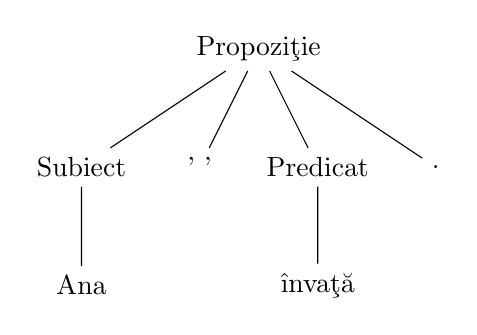
\begin{tikzpicture}
\node {Propoziţie}
child {node {Subiect} 
   child {node {Ana}}
}
child {node {' '}}
child {node {Predicat}
   child {node {învaţă}}
}
child {node {.}
};
\end{tikzpicture}
\caption{Arborele sintactic descendent pentru propoziţia \textit{Ana învaţă.}}
\end{figure}

Arborii sintactici sunt o reprezentare arborescentă a succesiunii de derivări prin care se generează o anumită propoziţie. Fiecare nod al arborelui care nu este frunză, este etichetat cu un neterminal. Fiecare frunză a arborelui este etichetată cu un terminal. 

Citind etichetele nodurilor arborelui (de la stânga la dreapta) de pe un nivel dat se obţine o formă propoziţională. 

\begin{figure}[H]
\centering
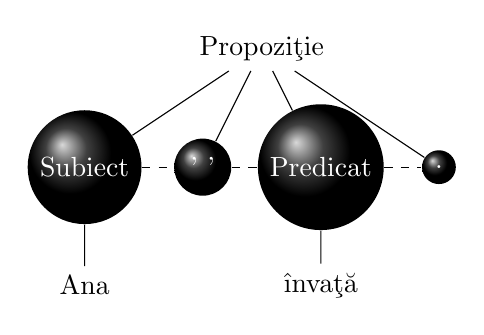
\begin{tikzpicture}
\node {Propoziţie}
child {node[ball color=black,circle,text=white] (1) {Subiect} 
   child {node {Ana}}
}
child {node[ball color=black,circle,text=white] (2) {' '}}
child {node[ball color=black,circle,text=white] (3) {Predicat}
   child {node {învaţă}}
}
child {node[ball color=black,circle,text=white] (4) {.}
};
\draw[dashed,-] (1) -- (2) -- (3) -- (4);
\end{tikzpicture}
\caption{Forma propoziţională \textit{Subiect ' ' Predicat .}}
\end{figure}

Citind etichetele frunzelor arborelui (de la stânga la dreapta) se obţine propoziţia pentru care a fost construit arborele.

\begin{figure}[H]
\centering
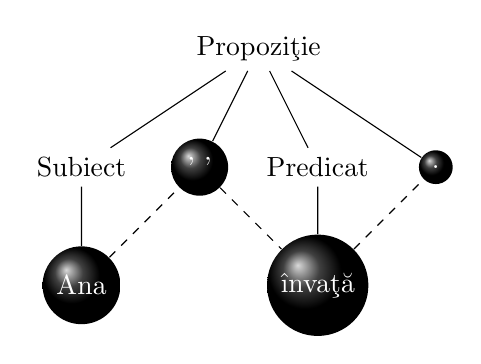
\begin{tikzpicture}
\node {Propoziţie}
child {node {Subiect} 
   child {node[ball color=black,circle,text=white] (1) {Ana}}
}
child {node[ball color=black,circle,text=white] (2) {' '}}
child {node {Predicat}
   child {node[ball color=black,circle,text=white] (3) {învaţă}}
}
child {node[ball color=black,circle,text=white] (4) {.}
};
\draw[dashed,-] (1) -- (2) -- (3) -- (4);
\end{tikzpicture} 
\caption{Propoziţia \textit{Ana învaţă.}}
\end{figure}

Construcţia arborelui sintactic pentru o propoziţie dată se poate face în două moduri. Se poate porni de la rădăcină către frunze, adică de la simbolul de start către propoziţie. Această manieră se numeşte construcţie descendentă. Sau se poate porni de la frunze către rădăcină, adică de la propoziţie către simbolul de start. Această manieră de construcţie se numeşte ascendentă.

Verificarea dacă o propoziţie dată aparţine limbajului definit de o gramatică formală se numeşte analiză sintactică. Ea constă în încercarea de a construi arborele sintactic al propoziţiei date, conform gramaticii care defineşte limbajul respectiv. Dacă se poate construi un arbore sintactic pentru propoziţie, atunci înseamnă că ea poate fi generată de către gramatică şi deci aparţine limbajului. Dacă nu se poate construi un astfel de arbore, atunci înseamnă că propoziţia nu aparţine limbajului. Dacă analiza încearcă construirea arborelui sintactic în maniera descendentă, atunci ea se numeşte analiză sintactică descendentă. Dacă încearcă construirea arborelui în sens ascendent, atunci se numeşte analiză sintactică ascendentă. Evident arborele sintactic descendent al unei propoziţii este identic cu arborele sintactic ascendent al aceleiaşi propoziţii.

Exemplu:

Arborele sintactic din exemplul precedent este un arbore sintactic descendent. Iată arborele sintactic ascendent pentru aceeaşi propoziţie.

\begin{figure}[H]
\centering
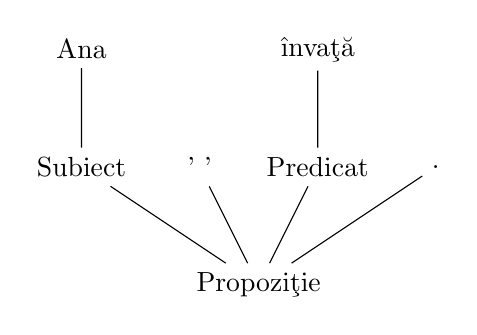
\begin{tikzpicture}
\node {Propoziţie}[grow=up]
child {node {.}}
child {node {Predicat}
   child {node {învaţă}}
}
child {node {' '}}
child {node {Subiect} 
   child {node {Ana}}
};
\end{tikzpicture}
\caption{Arborele sintactic ascendent pentru propoziţia \textit{Ana învaţă.}}
\end{figure}

\section{Exerciţii}

\textbf{Exerciţiul 1:}

Fie gramatica $G = (V_{N}, \Sigma, S, P)$. Determinaţi regulile de producţie, mulţimea terminalelor şi a neterminalelor şi simbolul de start, astfel încât gramatica să definească limbajul numerelor naturale.
\begin{itemize}
\item
$V_{N} = \{N,L_c,C\}$,
\item
$\Sigma = \{0,1,2,3,4,5,6,7,8,9\}$,
\item
$S$ este neterminalul $N$, 
\item
$P = \{$
\begin{itemize}
\item
$N \rightarrow L_c$,
\item
$L_c \rightarrow CL_c | C$,
\item
$C \rightarrow 0|1|2|3|4|5|6|7|8|9$
\end{itemize}
\}
\end{itemize}

Alfabetul limbajului este format din toate simbolurile care pot apărea în cadrul propoziţiilor limbajului, adică din toate cifrele de la 0 la 9.

Pentru construirea regulilor de producţie, am folosit următorul raţionament. Se cunoaşte că o gramatică defineşte sintaxa unui limbaj, adică forma propoziţiilor acestuia. Deci, ne-am pus întrebarea, cum arată propoziţiile din limbajul pentru care trebuie să construim gramatica? Aceste propoziţii sunt de fapt numerele naturale. Un număr natural este o succesiune de cifre formată din cel puţin o cifră (C). Deci forma propoziţiilor este cea a unei liste de cifre ($L_c$). Cum se poate defini o listă de cifre care poate să aibă o infinitate de elemente? Singurul mecanism pe care regulile de producţie ni-l pun la dispoziţie pentru a putea defini o succesiune infinită de simboluri este recursivitatea. Atunci trebuie să stabilim cum putem defini recursiv o listă de cifre. O listă de cifre este formată din primul ei element, care este o cifră, urmat de restul listei de cifre, care este tot o listă de cifre. Iar restul listei de cifre este format din primul său element, care este o cifră, urmat de restul restului listei de cifre, care este tot o listă de cifre, ş.a.m.d. până la ultimul element al listei, care este o listă de cifre format dintr-un singur element, adică o cifră. Prin urmare, cazul de bază al recursivităţii este faptul că cea mai simplă listă de cifre este formată dintr-o singură cifră (de unde a rezultat regula de producţie $L_c \rightarrow C$), iar formula de recurenţă este cea exprimată prin regula de producţie $L_c \rightarrow CL_c$. În plus, într-o gramatică, regulile de producţie ale simbolului de start vor arăta întotdeauna toate formele pe care le pot avea propoziţiile unui limbaj. În acest caz, este vorba de o singură formă ($N \rightarrow L_c$).

Următorul şir de derivări, care reprezintă generarea propoziţiei \textit{2573}, este format din derivări stânga.
\[ N \Rightarrow L_c \Rightarrow CL_c \Rightarrow 2L_c \Rightarrow2CL_c \Rightarrow25L_c \Rightarrow25CL_c \Rightarrow 257L_c \Rightarrow 257C \Rightarrow 2573 \]

Arborele sintactic descendent corespunzător propoziţiei este:

\begin{figure}[H]
\centering
\begin{tikzpicture}
\node {N}
child {node {$L_c$}
  child {node{C}
    child {node{2}}
  }
  child {node {$L_c$}
    child {node {C}
      child {node {5}}
    }
    child {node {$L_c$}
      child {node {C}
        child {node {7}}      
      }
      child {node {$L_c$}
        child {node {C}
          child {node {3}}        
        }
      }    
    }
  }
};
\end{tikzpicture} 
\caption{Arborele sintactic descendent pentru propoziţia \textit{2573}}
\end{figure}

Arborele sintactic ascendent corespunzător propoziţiei este:

\begin{figure}[H]
\centering
\begin{tikzpicture}
\node {N}[grow=up]
child {node {$L_c$}
  child {node {$L_c$}
    child {node {$L_c$}
      child {node {$L_c$}
        child {node {C}
          child {node {3}}        
        }
      }
      child {node {C}
        child {node {7}}      
      }    
    }
    child {node {C}
      child {node {5}}
    }
  }  
  child {node{C}
    child {node{2}}
  }
};
\end{tikzpicture}
\caption{Arborele sintactic ascendent pentru propoziţia \textit{2573}}
\end{figure}

Analizând gramatica definită mai sus, se poate constata că ea permite generarea numerelor de forma: orice succesiune de zerouri urmată de un număr natural oarecare (de exemplu 00013). Cum se poate modifica gramatica, astfel încât aceste propoziţii să nu mai poată fi generate? Oferim mai jos una dintre modalităţile în care se poate realiza acest lucru.

Fie gramatica $G = (V_{N}, \Sigma, S, P)$, astfel încât:

\begin{itemize}
\item
$V_{N} = \{N,L_c,C,D\}$,
\item
$\Sigma = \{0,1,2,3,4,5,6,7,8,9\}$,
\item
$S$ este neterminalul $N$, 
\item
$P = \{$
\begin{itemize}
\item
$N \rightarrow D L_c| C$,
\item
$Lc \rightarrow CL_c | C$,
\item
$C \rightarrow 0|1|2|3|4|5|6|7|8|9$
\item
$D \rightarrow 1|2|3|4|5|6|7|8|9$
\end{itemize}
\}
\end{itemize}

Următorul şir de derivări, care reprezintă generarea propoziţiei \textit{2573}, este format din derivări dreapta.

$ N \Rightarrow D L_c \Rightarrow DCL_c \Rightarrow DCCL_c \Rightarrow DCCC  \Rightarrow DCC3 \Rightarrow DC73 \Rightarrow D573 \Rightarrow 2573 $

Următorul şir de derivări, care reprezintă generarea propoziţiei \textit{2573}, este format din derivări stânga.

$ N \Rightarrow D L_c \Rightarrow 2L_c \Rightarrow2CL_c \Rightarrow 25L_c \Rightarrow 25CL_c \Rightarrow 257L_c \Rightarrow 257C \Rightarrow 2573$

Se observă că ambele tipuri de derivări, adică atât şirul derivărilor stânga, cât şi şirul derivărilor dreapta, pleacă de la aceeaşi formă propoziţională (adică de la simbolul de start) şi ajung la propoziţie. Diferenţa dintre cele două şiruri de derivări constă în formele propoziţionale intermediare, care sunt diferite.

Cu toate acestea arborele corespunzător propoziţiei, fie că este realizat folosind derivări dreapta, fie că este realizat folosind derivări stânga, este unic.

Gramatica de mai sus este o gramatică de tipul 2, adică este o gramatică independentă de context. Dacă limbajul pentru care a fost construită o gramatică este un limbaj regulat, atunci există cel puţin o gramatică regulată care să definească limbajul respectiv. Limbajul numerelor naturale este un limbaj regulat şi, prin urmare, se poate construi o gramatică regulată care să definească acest limbaj. Oferim mai jos o astfel de gramatică.

Fie gramatica $G = (V_{N}, \Sigma, S, P)$, astfel încât:

\begin{itemize}
\item
$V_{N} = \{N,L_c,C\}$,
\item
$\Sigma = \{0,1,2,3,4,5,6,7,8,9\}$,
\item
$S$ este neterminalul $N$, 
\item
$P = \{$
\begin{itemize}
\item
$N \rightarrow 1 L_c | 2 L_c | 3 L_c | 4 L_c | 5 L_c | 6 L_c | 7 L_c| 8 L_c | 9 L_c| C $,
\item
$Lc \rightarrow 0 L_c | 1 L_c | 2 L_c | 3 L_c | 4 L_c | 5 L_c | 6 L_c | 7 L_c| 8 L_c | 9 L_c | C$,
\item
$C \rightarrow 0|1|2|3|4|5|6|7|8|9$
\end{itemize}
\}
\end{itemize}

O proprietate interesantă a gramaticilor regulate este faptul că, pentru orice propoziţie din limbaj, şirul derivărilor stânga coincide cu şirul derivărilor dreapta. Acest lucru se datorează faptului că formele propoziţionale intermediare între simbolul de start şi propoziţie conţin un singur neterminal (deoarece la orice derivare se utilizează o singură regulă de producţie, iar partea dreaptă a regulilor de producţie ale unei gramatici regulate conţine un singur neterminal). Şi atunci, indiferent dacă înlocuim mai întâi neterminalul cel mai din stânga sau pe cel mai din dreapta, vom acţiona de fapt asupra aceluiaşi neterminal.

Următorul şir de derivări, care reprezintă generarea propoziţiei \textit{2573}, este format din derivări dreapta.

$ N \Rightarrow 2 L_c \Rightarrow 25L_c \Rightarrow 257L_c \Rightarrow 257C  \Rightarrow 2573$

Următorul şir de derivări, care reprezintă generarea propoziţiei \textit{2573}, este format din derivări stânga.

$ N \Rightarrow 2 L_c \Rightarrow 25L_c \Rightarrow 257L_c \Rightarrow 257C  \Rightarrow 2573$

Se observă că cele două şiruri de derivări sunt identice.

\textbf{Exerciţiul 2:}

Fie gramatica $G = (V_{N}, \Sigma, S, P)$. Scrieţi regulile de producţie, mulţimea terminalelor şi a neterminalelor şi determinaţi simbolul de start, astfel încât gramatica să definească limbajul numerelor întregi.

Fie gramatica $G = (V_{N}, \Sigma, S, P)$, astfel încât:

\begin{itemize}
\item
$V_{N}$ = \{N,$L_c$,C,D,Z\},
\item
$\Sigma$ = \{+, -, 0, 1, 2, 3,4,5,6,7,8,9\},
\item
S este neterminalul N,
\item
$P = \{$
\begin{itemize}
\item
$N \rightarrow ZDL_c | ZC$,
\item
$L_c \rightarrow CL_c | C$,
\item
C $\rightarrow$ $0|1|2|3|4|5|6|7|8|9$
\item
D $\rightarrow$ $1|2|3|4|5|6|7|8|9$
\item
Z $\rightarrow$  $+|-$
\end{itemize}
\}
\end{itemize}

Alfabetul limbajului este format din toate simbolurile care pot apărea în cadrul propoziţiilor limbajului, adică din toate cifrele de la 0 la 9 şi cele două semne posibile, plus şi minus.

În construcţia regulilor de producţie s-a procedat la fel ca şi în exemplul anterior. S-a plecat de la forma propoziţiilor din limbajul de definit: numerele întregi sunt numere naturale cu semn. Având deci ca punct de plecare gramatica exemplului anterior, s-a adăugat neterminalul $Z$ care reprezintă semnul numărului, neterminal care a fost folosit la începutul părţii drepte a tuturor regulilor de producţie ale simbolului de start.

Următorul şir de derivări, care reprezintă generarea propoziţiei \textit{-50}, este format din derivări stânga.

$ N \Rightarrow ZDLc \Rightarrow -DLc \Rightarrow -5Lc \Rightarrow -5C \Rightarrow -50$ 

Care este şirul derivărilor dreapta, pentru aceeaşi propoziţie?

Arborele sintactic descendent corespunzător propoziţiei este:

\begin{figure}[H]
\centering
\begin{tikzpicture}
\node {N}
child {node {Z}
  child {node {-}}
}
child {node {D}
  child {node {5}}
}
child {node {$L_c$}
  child {node {C}
    child {node {0}}  
  }
}
;
\end{tikzpicture} 
\caption{Arborele sintactic descendent pentru propoziţia \textit{-50}}
\end{figure}

Care este arborele sintactic ascendent corespunzător aceleiaşi propoziţii?

Care este tipul acestei gramatici? Construiţi o gramatică regulată care să definească acelaşi limbaj (limbajul numerelor întregi este un limbaj regulat).

\textbf{Exerciţiul 3:}

Fie gramatica $G = (V_{N}, \Sigma, S, P)$. Determinaţi regulile de producţie, mulţimea terminalelor şi a neterminalelor şi simbolul de start, astfel încât gramatica să definească limbajul numerelor raţionale.

Fie gramatica $G = (V_{N}, \Sigma, S, P)$, astfel încât:

\begin{itemize}
\item
$V_{N}$ = \{P,N,M,$L_c$,C,D,Z\},
\item
$\Sigma$ = \{+, -, /, 0, 1, 2, 3,4,5,6,7,8,9\},
\item
S este neterminalul P,
\item
$P = \{$
\begin{itemize}
\item
P $\rightarrow$  N/M,
\item
$N \rightarrow ZDL_c | 0 | ZD$,
\item
$M \rightarrow ZDL_c | ZD$,
\item
$L_c \rightarrow CL_c | C$,
\item
C $\rightarrow$ $0|1|2|3|4|5|6|7|8|9$
\item
D $\rightarrow$ $1|2|3|4|5|6|7|8|9$
\item
Z $\rightarrow$  $+|-$
\end{itemize}
\}
\end{itemize}

Alfabetul limbajului este format din toate simbolurile care pot apărea în cadrul propoziţiilor limbajului, adică din toate cifrele de la 0 la 9, semnele plus şi minus şi semnul de fracţie.

Punctul de plecare pentru enumerarea acestor elemente a fost sintaxa propoziţiilor limbajului de definit. O propoziţie a limbajului (adică un număr raţional) este de forma $n/m$, unde n şi m sunt numere întregi, iar m este diferit de zero. De aici rezultă regula de producţie pentru simbolul de start ($P \rightarrow  N/M$), precum şi regulile de producţie pentru celelalte neterminale.

Următorul şir de derivări, care reprezintă generarea propoziţiei \textit{-51/-301}, este format din derivări dreapta.

$ P \Rightarrow N/M  \Rightarrow N/ZDL_c  \Rightarrow N/ZDCL_c \Rightarrow N/ZDCC \Rightarrow N/ZDC1 \Rightarrow N/ZD01 \Rightarrow N/Z301 \Rightarrow  N/-301 \Rightarrow ZDL_c/-301 \Rightarrow ZDC/-301 \Rightarrow ZD1/-301 \Rightarrow Z51/-301 \Rightarrow -51/-301$

Care este şirul derivărilor stânga, pentru aceeaşi propoziţie?

Arborele sintactic ascendent corespunzător propoziţiei este:

\begin{figure}[H]
\centering
\begin{tikzpicture}
%\tikzset{level 1/.style={level distance=0.5cm}}
\tikzset{level 1/.style={sibling distance=20mm}}
\tikzset{level 2/.style={sibling distance=10mm}}
\node {P}[grow=up]
child {node {M}
  child {node {$L_c$}
     child {node {$L_c$}
       child {node {C}
         child {node {1}}       
       }     
     }
     child {node {C}
       child {node {0}}
     }   
   }
   child {node {D}
     child {node {3}}   
   }
   child {node {Z}
     child {node {-}}   
   } 
}
child {node {/}}
child {node{N}
  child {node {$L_c$}
     child {node {C}
       child {node {1}}     
     }   
   }
   child {node {D}
     child {node {5}}   
   }
   child {node {Z}
     child {node {-}}   
   }
}
;
\end{tikzpicture}
\caption{Arborele sintactic ascendent pentru propoziţia \textit{-51/-301}}
\end{figure}

Care este arborele sintactic descendent corespunzător aceleiaşi propoziţii?

Care este tipul acestei gramatici? Construiţi o gramatică regulată care să definească acelaşi limbaj (limbajul numerelor raţionale este un limbaj regulat).

\textbf{Exerciţiul 4:}

Fie gramatica $G = (V_{N}, \Sigma, S, P)$. Enumeraţi regulile de producţie, mulţimea terminalelor şi a neterminalelor şi determinaţi simbolul de start, astfel încât gramatica să definească limbajul numerelor reale.

Fie gramatica $G = (V_{N}, \Sigma, S, P)$, astfel încât:

\begin{itemize}
\item
$V_{N}$ = \{R,N,M,$L_c$,C,D,Z\},
\item
$\Sigma$ = \{+, -, ., 0, 1, 2, 3,4,5,6,7,8,9\},
\item
S este neterminalul R,
\item
$P = \{$
\begin{itemize}
\item
R $\rightarrow$  N.M,
\item
$N \rightarrow ZDL_c | ZD | Z0$,
\item
$M \rightarrow L_c |C$,
\item
$Lc \rightarrow CL_c | C$,
\item
C $\rightarrow 0|1|2|3|4|5|6|7|8|9$
\item
D $\rightarrow 1|2|3|4|5|6|7|8|9$
\item
Z $\rightarrow$  $+|-$
\end{itemize}
\}
\end{itemize}

Alfabetul limbajului este format din toate simbolurile care pot apărea în cadrul propoziţiilor limbajului, adică din toate cifrele de la 0 la 9, semnele plus şi minus şi punctul.

Sintaxa propoziţiilor limbajului (sintaxa numerelor reale) este cea care ne ajută să definim elementele gramaticii. Un număr real este format din partea întreagă şi partea zecimală, separate prin simbolul punct; partea întreagă este un număr întreg, iar partea zecimală este o listă oarecare de cifre. De aici rezultă expresia regulii de producţie pentru simbolul de start, precum şi pentru regulile de producţie ale celorlalte neterminale.

Următorul şir de derivări, care reprezintă generarea propoziţiei \textit{-123.089}, este format din derivări stânga.

$ R \Rightarrow N.M  \Rightarrow ZDL_c.M  \Rightarrow -1CL_c.M \Rightarrow -12C.M \Rightarrow -123.M \Rightarrow-123.L_c \Rightarrow -123.CL_c \Rightarrow -123.0CL_c \Rightarrow-123.09C \Rightarrow -123.098$ 

Care este şirul derivărilor dreapta, pentru aceeaşi propoziţie?

Arborele sintactic descendent corespunzător propoziţiei este:

\begin{figure}[H]
\centering
\begin{tikzpicture}
%\tikzset{level 1/.style={level distance=5cm}}
\tikzset{level 1/.style={sibling distance=20mm}}
\tikzset{level 2/.style={sibling distance=10mm}}
\node {R}
child {node{N}
  child {node {Z}
    child {node {-}}  
  }
  child {node {D}
    child {node {1}}  
  }
  child {node {$L_c$}
    child {node {C}
      child {node {2}}    
    }  
    child {node {$L_c$}
      child {node {C}
        child {node {3}}      
      }    
    }
  }
}
child {node {.}}
child {node {M}
  child {node {$L_c$}
    child {node {C} 
      child {node {0}}   
    }
    child {node {$L_c$}
      child {node {C}
        child {node {9}}      
      }    
      child {node {$L_c$}
        child {node {C}
          child {node {8}}        
        }      
      }
    }  
  }
}
;
\end{tikzpicture} 
\caption{Arborele sintactic descendent pentru propoziţia \textit{-123.089}}
\end{figure}

Care este arborele sintactic ascendent corespunzător aceleiaşi propoziţii?

Care este tipul acestei gramatici? Construiţi o gramatică regulată care să definească acelaşi limbaj (limbajul numerelor reale este un limbaj regulat).

\textbf{Exerciţiul 5:}

Fie gramatica $G = (V_{N}, \Sigma, S, P)$. Enumeraţi regulile de producţie, mulţimea terminalelor şi a neterminalelor şi determinaţi simbolul de start, astfel încât gramatica să definească limbajul numerelor reale scrise folosind separatorul de mii (virgula).

Fie gramatica $G = (V_{N}, \Sigma, S, P)$, astfel încât:

\begin{itemize}
\item
$V_{N}$ = \{R,N,M,$L_c$,C,D,Z\},
\item
$\Sigma$ = \{+, -, . , , , 0, 1, 2, 3, 4, 5, 6, 7, 8, 9\},
\item
S este neterminalul R,
\item
$P = \{$
\begin{itemize}
\item
R $\rightarrow$ ZN.M,
\item
N $\rightarrow$ D,G | DC,G| DCC,G | D | DC | DCC | 0,
\item
G $\rightarrow$ CCC | G.CCC,
\item
$M \rightarrow L_c |C$,
\item
$L_c \rightarrow CL_c | C$,
\item
C $\rightarrow$ $0|1|2|3|4|5|6|7|8|9$
\item
D $\rightarrow$ $1|2|3|4|5|6|7|8|9$
\item
Z $\rightarrow$  $+|-$
\end{itemize}
\}
\end{itemize}

Următorul şir de derivări, care reprezintă generarea propoziţiei \textit{-1,003.8}, este format din derivări stânga.

$ R \Rightarrow ZN.M  \Rightarrow -D,G.M  \Rightarrow -1,CCC.M \Rightarrow -1,003.M \Rightarrow -1,003.C \Rightarrow -1,003.8$ 

Următorul şir de derivări, care reprezintă generarea propoziţiei \textit{-1,000,000.35}, este format din derivări stânga.

$ R \Rightarrow ZN.M  \Rightarrow -N.M  \Rightarrow -D,G.M \Rightarrow -D,G,CCC.M \Rightarrow -D,CCC,CCC.M \Rightarrow -1,000,000.L_c \Rightarrow -1,000,000.CL_c \Rightarrow -1,000,000.3C \Rightarrow -1,000,000.35$ 

Care sunt şirurile derivărilor dreapta, pentru cele două propoziţii?

Arborele sintactic ascendent corespunzător primei propoziţiei este:

\begin{figure}[H]
\centering
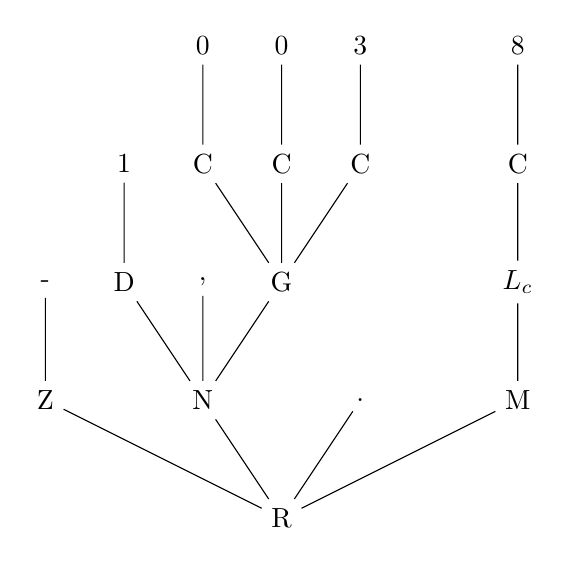
\begin{tikzpicture}
\tikzset{level 1/.style={sibling distance=20mm}}
\tikzset{level 2/.style={sibling distance=10mm}}
\node {R}[grow=up]
child {node {M}
  child {node {$L_c$}
    child {node {C}
      child {node {8}}
    }
  }
}
child {node {.}}
child {node {N}
  child {node {G}
     child {node {C}
       child {node {3}}
     }
     child {node {C}
       child {node {0}}     
     }  
     child {node {C}
       child {node {0}}     
     }
  }
  child {node {,}}
  child {node {D}
    child {node {1}}  
  }
}
child {node {Z}
  child {node {-}}
}  
;
\end{tikzpicture}
\caption{Arborele sintactic ascendent pentru propoziţia \textit{-1.003,8}}
\end{figure}

Care este arborele sintactic descendent corespunzător aceleiaşi propoziţii?

\textbf{Exerciţiul 6:}

Pornind de la următorul exemplu de program, să se construiască o gramatică care să definească un limbaj de programare care să permită scrierea de programe cu structura şi instrucţiunile regăsite în exemplu.

int $a=3$;		
\newline
float b; 		
\newline
program test	
\newline
begin			
\newline
float c;		
\newline
$c=a*b+6.0$;	
\newline
print c;		
\newline
end				

Se observă că limbajul permite stabilirea numelui programului, delimitarea corpului programului prin cuvintele "begin" şi "end", declararea de variabile globale (înainte de linia "program test") sau locale, cu sau fără iniţializarea valorii acestora, utilizarea expresiilor aritmetice, instrucţiuni de atribuire, afişarea valorii unei variabile.

Definirea limbajului de programare pentru care programul de mai sus este un exemplu, se va face în două etape: \textbf{definirea lexicului (vocabularului)} şi \textbf{definirea sintaxei}. Pentru ambele etape se vor folosi gramaticile formale.

Definirea lexicului constă în definirea atomilor lexicali care pot apărea în propoziţiile limbajului. Atomii lexicali reprezintă cele mai mici unităţi componente ale unei propoziţii care au sens prin ei înşişi. Ei constă din succesiuni de simboluri formate de baza alfabetului limbajului (literele mici şi mari, cifrele, alte simboluri cu caracter special). În mod asemănător vorbim despre lexicul sau vocabularul unei limbi care reprezintă toate cuvintele care fac parte din limba respectivă. Aceste cuvinte sunt succesiuni de simboluri din mulţimea alfabetului limbii şi constituie de fapt atomii lexicali ai limbii respective, fiind cele mai mici unităţi de vorbire care au sens. Ea se va face prin definirea a câte unei gramatici pentru fiecare dintre categoriile lexicale care pot apărea în cadrul limbajului:

\begin{enumerate}
\item
cuvinte cheie: int, float, program, begin, end, print.
\item
identificatori (numele programului şi numele variabilelor). Această categorie conţine o infinitate de elemente şi anume toate succesiunile de simboluri formate din litere şi cifre care încep cu o literă. De aceea pentru a reprezenta un identificator se va folosi simbolul "ID", care însă este un terminal, iar nu un neterminal, deoarece ţine loc oricărui element din mulţimea infinită a numelor posibile. Practic categoria identificatorilor este ea însăşi un limbaj în sine, ale cărui propoziţii se notează cu "ID".

Gramatica care defineşte identificatorii este $G_1 = (V_{N}, \Sigma, S, P)$, astfel încât:

\begin{itemize}
\item
$V_{N} = \{ID,Li,L,C\}$,
\item
$\Sigma$ = \{a, b, $\dots$ , z, A, B, $\dots$, Z, 0, 1, $\dots$, 9\},
\item
S este neterminalul ID,
\item
$P = \{$
\begin{itemize}
\item
ID $\rightarrow$ L | LLi
\item
Li $\rightarrow$ LLi | CLi | L | C
\item
L $\rightarrow$ a | b | $\dots$ | z | A | B | $\dots$ | Z
\item
C $\rightarrow$ 0 | 1 | $\dots$ | 9
\end{itemize}
\}
\end{itemize}

\item
operatori: =, +, -, *, $/$.
\item
semne de punctuaţie: ;, spaţiul (Linia nouă nu va fi luată în considerare, deoarece faptul că programul este scris pe mai multe linii sau pe o singură linie nu are importanţă. Scrierea pe mai multe linii are doar avantajul de a oferi o lizibilitate mărită.)
\item
constantele
\begin{enumerate}
\item
constante de tip numere întregi. Această categorie conţine un număr foarte mare de elemente şi anume toate numere întregi care pot fi reprezentate pe un număr de octeţi egal cu cel folosit pentru a stoca astfel de valori. De aceea pentru a reprezenta o constantă întreagă se va folosi simbolul "CTI", care însă este un terminal, iar nu un neterminal, deoarece ţine loc oricărui element din mulţimea numerelor întregi reprezentabile. Practic şi categoria constantelor întregi este ea însăşi un limbaj în sine, ale cărui propoziţii se notează cu "CTI".

Gramatica care defineşte constantele de tip numere întregi este $G_2 = (V_{N}, \Sigma, S, P)$, astfel încât:

\begin{itemize}
\item
$V_{N}$ = \{CTI,$L_c$,C,D,Z\},
\item
$\Sigma$ = \{+, -, 0, 1, 2, 3,4,5,6,7,8,9\},
\item
S este neterminalul CTI,
\item
$P = \{$
\begin{itemize}
\item
$CTI \rightarrow ZDL_c | ZC$,
\item
$L_c \rightarrow CL_c | C$,
\item
C $\rightarrow$ $0|1|2|3|4|5|6|7|8|9$
\item
D $\rightarrow$ $1|2|3|4|5|6|7|8|9$
\item
Z $\rightarrow$  $+|-$
\end{itemize}
\}
\end{itemize}

\item
constante de tip numere reale. Această categorie conţine un număr foarte mare de elemente şi anume toate numere reale care pot fi reprezentate pe un număr de octeţi egal cu cel folosit pentru a stoca astfel de valori. De aceea pentru a reprezenta o constantă reală se va folosi simbolul "CTR", care însă este un terminal, iar nu un neterminal, deoarece ţine loc oricărui element din mulţimea numerelor reale reprezentabile. Practic şi categoria constantelor reale este ea însăşi un limbaj în sine, ale cărui propoziţii se notează cu "CTR".

Gramatica care defineşte constantele de tip numere reale este $G_3 = (V_{N}, \Sigma, S, P)$, astfel încât:

\begin{itemize}
\item
$V_{N}$ = \{CTR,N,M,$L_c$,C,D,Z\},
\item
$\Sigma$ = \{+, -, ., 0, 1, 2, 3,4,5,6,7,8,9\},
\item
S este neterminalul CTR,
\item
$P = \{$
\begin{itemize}
\item
R $\rightarrow$  N.M,
\item
$N \rightarrow ZDL_c | ZD | Z0$,
\item
$M \rightarrow L_c |C$,
\item
$Lc \rightarrow CL_c | C$,
\item
C $\rightarrow 0|1|2|3|4|5|6|7|8|9$
\item
D $\rightarrow 1|2|3|4|5|6|7|8|9$
\item
Z $\rightarrow$  $+|-$
\end{itemize}
\}
\end{itemize}

\end{enumerate}
\end{enumerate}

Definirea sintaxei limbajului constă în definirea modului în care elementele lexicului (adică atomii lexicali) se grupează împreună pentru a forma propoziţiile limbajului. 

Gramatica care defineşte sintaxa limbajului este $G = (V_{N}, \Sigma, S, P)$, astfel încât:

\begin{itemize}
\item
$V_{N} = \{Lg,P,D,Li,E,I,C,S\}$,
\item
$\Sigma$ = \{int, float, program, begin, end, =, ; , print, ID,  , CTI, CTR, +, -, *, /\},
\item
S este neterminalul S,
\item
$P = \{$
\begin{itemize}
\item
S $\rightarrow$ LgP | P
\item
Lg $\rightarrow$ LgD; | D;
\item
D $\rightarrow$ int ID | int ID=CTI | float ID | float ID=CTR
\item
P $\rightarrow$ program ID begin Li end
\item
Li $\rightarrow$ LiI; | I;
\item
I $\rightarrow$ D | ID=E | print ID
\item
E $\rightarrow$ E + E | E - E | E * E | E / E | ID | CTI | CTR
\end{itemize}
\}
\end{itemize}

Se observă că în definirea alfabetului gramaticii care defineşte sintaxa limbajului au fost enumerate în mod direct elementele lexicale finite (cuvintele cheie, operatorii, semnele de punctuaţie), iar elementele lexicale infinite ca şi număr (identificatori şi constate) au fost reprezentate prin simbolul de start al gramaticii care le defineşte, conform explicaţiilor de mai sus.

Următorul şir de derivări, care reprezintă generarea propoziţiei dată ca şi exemplu, este format din derivări dreapta.

\textbf{\underline{S}} $\rightarrow$ 

\textbf{Lg\underline{P}} $\rightarrow$ 

Lg \textbf{program ID begin \underline{Li} end} $\rightarrow$ 

Lg program ID begin \textbf{Li \underline{I} ;} end $\rightarrow$

Lg program ID begin \underline{Li} \textbf{print ID} ; end $\rightarrow$ 

Lg program ID begin \textbf{Li \underline{I} ;} print ID ; end $\rightarrow$

Lg program ID begin Li \textbf{ID = \underline{E}} ; print ID ; end $\rightarrow$

Lg program ID begin Li ID = \textbf{E + \underline{E}} ; print ID ; end $\rightarrow$

Lg program ID begin Li ID = \underline{E} + \textbf{CTR} ; print ID ; end $\rightarrow$

Lg program ID begin Li ID = \textbf{E * \underline{E}} + CTR ; print ID ; end $\rightarrow$

Lg program ID begin Li ID = \underline{E} * \textbf{ID} + CTR ; print ID ; end $\rightarrow$

Lg program ID begin \underline{Li} ID = \textbf{ID} * ID + CTR ; print ID ; end $\rightarrow$

Lg program ID begin \textbf{\underline{I} ;} ID = ID * ID + CTR ; print ID ; end $\rightarrow$

Lg program ID begin \textbf{\underline{D}} ; ID = ID * ID + CTR ; print ID ; end $\rightarrow$

\underline{Lg} program ID begin \textbf{float ID} ; ID = ID * ID + CTR ; print ID ; end $\rightarrow$

\textbf{Lg \underline{D} ;} program ID begin float ID ; ID = ID * ID + CTR ; print ID ; end $\rightarrow$

\underline{Lg} \textbf{float ID} ; program ID begin float ID ; ID = ID * ID + CTR ; print ID ; end $\rightarrow$

\textbf{\underline{D} ;} float ID ; program ID begin float ID ; ID = ID * ID + CTR ; print ID ; end $\rightarrow$

\textbf{int ID = CTI} ; float ID ; program ID begin float ID ; ID = ID * ID + CTR ; print ID ; end

Care este şirul derivărilor stânga, pentru aceeaşi propoziţie?

Arborele sintactic descendent corespunzător propoziţiei este:

\begin{figure}[H]
\begin{tikzpicture}
\centering
\node {S}
child [sibling distance=5cm] {node  {Lg}
    child [sibling distance = 2cm]{node{Lg}
	child  [ sibling distance = 1cm]{node {D}
                   child[sibling distance = 1cm]{node{int}}
		child{node{ID}}
		child{ node{=}}
		child{node{CTI}}}
	child[sibling distance=1cm]{node{;}} }
    child [sibling distance = 2cm]{node{D}
	child{node{float}}
 	child[sibling distance = 2cm]{node{ID}}}
    child[sibling distance=2cm]{node{;}}}
child [sibling distance = 5cm] {node {P}
	child[sibling distance = 1cm]{node{program}}
	child[sibling distance = 1cm]{node{ID}}
	child{node{begin}}
	child[sibling distance = 1cm]{node{Li}
		child[sibling distance=3cm]{node{Li}
			child[sibling distance=2cm]{node{Li}
				child {node{I}
					child{node{D}
						child{node{float}}
						child{node{ID}}}}
				child[sibling distance=1cm]{node{;}}}
			child[sibling distance = 1cm]{node{I}
				child{node{ID}}
				child{node{=}}
				child[sibling distance = 1cm]{node{E}
					child{node{E}
						child{node{E}
							child{node{ID}}}
						child{node{*}}
                                                                child{node{E}
							child{node{ID}}}}
					child{node{+}}
					child{node{E}
						child{node{CTR}}}}}
			child[sibling distance=1.7cm]{node{;}}}
		child[sibling distance=2cm]{node{I}
			child[sibling distance=1cm]{node{print}}
			child[sibling distance=1cm]{node{ID}}}
		child[sibling distance=2.5cm]{node{;}}}
	child[sibling distance=1cm]{node{end}}};
\end{tikzpicture}
\caption{Arborele sintactic descendent pentru programul luat ca şi exemplu}
\end{figure}

Care este arborele sintactic ascendent corespunzător aceleiaşi propoziţii?

\section{Exerciţii propuse}

